% Developed architecture / system design / implementation:
% start with a theoretical approach
% describe the developed system/algorithm/method from a high-level point of view
% go ahead in presenting your developments in more detail

\chapter{Design}\label{ch:design}\glsresetall
% Our application is building entirely on decision making. If it seems like a \ac{pd} is coming up, buy, then sell on profit. Otherwise, wait for a \ac{pd}. Simple, yet effective if and only if the application can make accurate predictions. Our prediction algorithm needs to either detect \acp{pd} before it happens or exactly when it begins, because of the period where \ac{pd} peak span from seconds to max $10$ minutes as described in \autoref{sec:pd}. Are we too late with buying assets we may end up buying at or right before the peak which will result in a substantial loss because of the forthcoming dump. However, if we can manage to purchase assets just a few seconds in or before the \ac{pd} starts we can profit well by selling only a short time later when the coin peaks.

% For the application to have the ability to make accurate predictions, we need to carefully define a suitable algorithmic model that fits currently existing data to reverse engineer \acp{pd}. We find two paradigms \emph{financial} and \emph{\ac{ml}} as appealing fields for finding suitable algorithmic models. We encounter some problems in the field of finance, typically, financial institutions do not share their algorithms for competitive reasons, and we can not either find any models that are compatible for detecting \ac{pd} in real-time on cryptocurrency exchanges. We believe that using \ac{ml} to detect \acp{pd} is currently the optimal solution, and to reinforce that assumption, a recent PwC\footnote{Price Waterhouse Coopers is the largest network of accountants, lawyers and advisors, and deliver services within audit, consulting and tax.} study found that over the next two to three years \ac{ml} are the single most crucial technology impacting the finance function~\cite{pwc} as \ac{ml} models seem to excel financial models.

%XXX Explaining ML => background
% In recent years, \ac{ml} has become a buzzword and categorized as state of the art and "the solution" for every kind of problem, but it is important to remember that \ac{ml} is not always the optimal solution for every type of problem. There are certain cases where rule-based solutions perform better than \ac{ml}, cases, where we can directly predict values by using simple rules, computations, or predetermined steps that are easily programmable~\cite{aws}. So when should we use \ac{ml}? According to \cite{aws}, we should use \ac{ml} in following situations:
% \begin{itemize}
    % \item When tasks cannot be adequately solved using deterministic rule-based solutions. A considerable number of factors like features, patterns, correlated features, etc., can influence the answer. When rules depend on too many factors, and many of these rules overlap or need to be tuned very finely, it quickly becomes complicated to define these rules accurately.
    % \item When tasks do not scale, e.g., manual detection of spam mail which will be a tedious process if there are millions of emails. \ac{ml} solutions are effective at handling large-scale problems.
% \end{itemize}

% Looking at the amount of data that cryptocurrency exchanges and other cryptocurrency sources continuously produce, defining a \ac{ml} model is way more tempting than defining a rule-based solution. There are too much data and various types of data that currently exists that makes ruled-based solutions infeasible.

% Supervised learning problem
% binary classification problem
% Pump are anomalies
% choosing a model

% Moving on with \ac{ml}, we can define detection of \ac{pd} as a supervised \emph{binary classification} problem, \ac{pd} or not \ac{pd}. As with every supervised problem we need data that is labeled which are struggling to get.


% Our application only requires the knowledge of the pump part in a \ac{pd} to function. Our application wants to buy before or at the beginning of a pump and sell when the coin peak.

% Our application only requires the knowledge of the pump part in a \ac{pd}, as our application want to buy before or at the beginning of a pump and sell when the coin peak. We can ignore the dump part because it do not affect the decision made by our application. We can define this as a \emph{binary classification} problem, pump or not pump, or from our application perspective buy or sell.

% \acp{pd} are a common price manipulation scheme one observe on cryptocurrency exchanges, but in vast amount of existing data that exchanges produce a \ac{pd} is an \emph{anomaly}. It exist way more regular data than \ac{pd} data. This becomes problem when we want to  create a dataset containing regular data and \ac{pd} data because of the huge imbalance between the two classes, and \acp{pd} are rare entities hence it is also challenging to obtain a significant amount of \acp{pd} required to train a \ac{ml} model.

% Choosing a \ac{ml} model primarily depends on the nature of the input data. Input data can be broadly classified into sequential (e.g., voice, text, music, time series, protein sequences) or non-sequential data (e.g., images, other data)~\cite{dl_anomaly}. Cryptocurrency sources produce sequential data, more specifically \emph{time series} data. Time series data are linearly ordered sequence of values of a variable at equally spaced time intervals~\cite{stat_handbook}. 

% Anomaly detection in sequential data has attracted significant interest in the literature due to its applications in a wide range of engineering problems. \ac{lstm} neural network based algorithms for anomaly detection have been investigated and reported to produce significant performance gains over conventional methods  (Ergenet al. [2017]).

% Supervised anomaly detection techniques are superior in performance compared to unsupervised anomaly detection techniques since these techniques use labeled samples (G ̈ornitz et al. [2013]).  Supervised anomaly detection learnsthe separating boundary from a set of annotated data instances (training) and then, classify a test instance into eithernormal or anomalous classes with the learned model (testing).

% Moreover, the performance of deep supervised classifier used an anomaly detector is sub-optimal due to class imbalance (the total number of positive class instances are far more than the total number of negative class of data)~\cite{dl_anomaly}.

% Labels indicate whether a chosen data instance is normal or an outlier. Anomalies are rare entities hence it is challenging to obtain their labels~\cite{dl_anomaly}.
TBW
\section{Architectural overview}
We are modeling \project as a \ac{ml} pipeline, but with some few extensions. It is designed to extract raw data from different cryptocurrency sources and transform it into valuable information in order to classify \acp{pd}. The term \ac{ml} pipeline can be misleading as it implies a one-way flow of data when some elements in the pipeline are cyclical and iterative where every iteration intends to improve the accuracy of the model~\cite{ml_pipeline_3}. A pipeline provides many advantages, and according to \cite{ml_pipeline_2} some of them are.

\begin{itemize}
    \item \textbf{Flexibility} - Processing elements are easy to replace and to modify without changing the system.
    \item \textbf{Extensibility} - The system is partitioned into pieces making it easy to add new functionality.
    \item \textbf{Scalability} – Each processing element is separately scalable because they are independent.
\end{itemize}

\begin{figure}[ht]
    \centering
    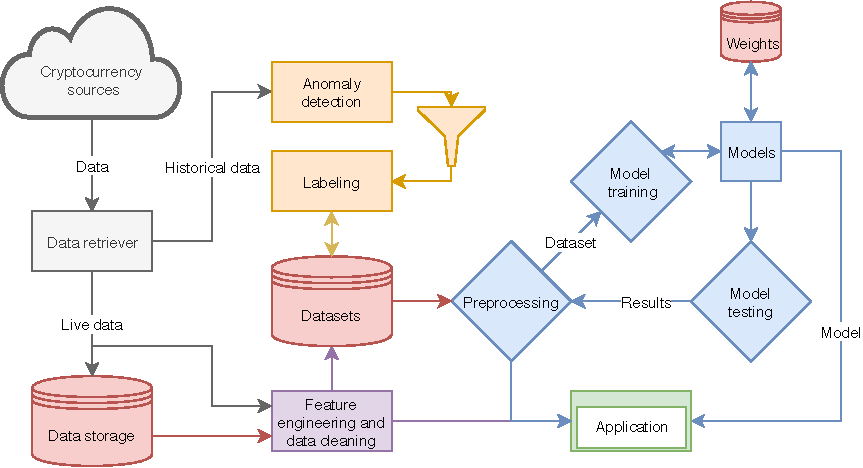
\includegraphics[width=\textwidth]{overview.pdf}
    \caption{Architectural overview of \project}
    \label{fig:overview}
\end{figure}

\project's pipeline consists of multiple stages, the coloring of each layer in \autoref{fig:overview} characterize each step.

The first step in the pipeline, pulls data from various cryptocurrency sources. The data is mostly incomplete and lacks behaviors or trends making it currently pointless to train a model with. This process is tedious because sources tend to have different request rates, \acp{api}, and the data can have various formats like \ac{json} or \ac{xml}.

The next step branches the retrieved data in two, live and historical data. Since we are trying to detect \acp{pd} in real-time we need to store live data continuously. When "captured" a compelling amount of \acp{pd} in the stored live data, we use an anomaly detection algorithm~\cite{P&D_to_the_moon} to detect \ac{pd} in the gathered live data. The anomaly detection algorithm is not compliant with live data, so we need to pull aggregated historical data that span over the period of the collected live data. As previously mentioned, anomaly detection algorithms tend to have a high false positive rate. Thus, we need to remove the false positive and keep the true positive manually.

The input data ultimately determine the performance of a \ac{ml} deep learning model~\cite{mike_voets}, so training a model with the raw gathered live data is ineffective. Hence, we need to define new convenient data set containing features created by processing the collected live data; this is a highly critical process and will later determine the classification performance of the deep learning model. The gathered live data also need to go through a cleansing process as it most likely contains irrelevant information that has nothing to with \acp{pd}.

With filtered anomalies containing \ac{pd} and a dataset, we can create a labeled dataset and train our model. Obtaining good classification results depends, as mentioned, on the features, but also how we decide to preprocess the dataset. Typical preprocessing strategies include dimensionality reduction and normalization. Having a labeled preprocessed dataset we can finally begin to the train the deep learning model, this a cyclical and a long process, as it requires many trial and error attempts to find the optimal weights for the model. In each cycle, we store the model's weights because it's not always the case that each iteration will improve the classification performance of the model.

For applications to utilize \project, they need to select a model and let live data flow through the same processing stages as the dataset that was used to train the model.

\section{Internal Components}
TBW

\subsection{Retrieving Data}
% Since we want to detect \acp{pd} on exchanges in real-time, the nature of the data we want to make classifications on must be real-time fine-grained data, so that we can detect \acp{pd} as early and accurate as possible. Aggregated historical data is too coarse-grained because exchanges generally only allow a discrete time interval selection of data where the smallest is typically one minute. The duration where a \ac{pd} start to its peak vary from a few seconds to max ten minutes~\cite{P&D_MIT_crypto, P&D_to_the_moon}, so the ability to make accurate predictions with one-minute data is questionable.

% Training a model in real-time by pulling data is impractical because we don't have any labels, and sources can only produce a limited amount of data at a time which will create a bottleneck of data supply to the model. To cope with this problem, we have to pull and store current live data continuously; this is an endless dreary process because we have to wait weeks until we have "captured" enough \acp{pd} events in our collected data to start training. If anything fails, we may have to start all over again because we are missing out on trends, which results in noisy data.

% From the reinforcers field in \autoref{tab:pd_indicators}, to reverse engineer \acp{pd}, we have to fetch data from various sources. An exchange alone do not produce data regarding a coin's capitalization nor if other exchanges list a specific coin. Other sources than exchanges produce such metadata of coins.

% We also have to ensure that the fetched data is at equally spaced interval in order to obtain clean data, and when training ,

Retrieving data from multiple cryptocurrency sources requires synchronization, 






% writing every n second
% Master slave
% synch or async?
% why? i/o bound
% intro
% which exchange to extract data from 
% BTC market
% ohlcv, depth
% describe features

\subsection{Detecting Pump-and-Dumps using an anomaly detection algorithm}
Manually collecting \ac{pd} events from chat applications to label our datasets, seems infeasible in the long run — even tough Livshits and Xu \cite{P&D_anatomy} hand-picked $220$ pump-events from July to November in 2018 from $358$ different Telegram groups to train a Random Forest. They still did miss out on plenty of other executed \ac{pd} schemes as there are numerous of other chatting applications and private organizers~\cite{blockonomi}. Also, searching for \ac{pd} events is a time-consuming process, and incorrect labeling occurs when we lack membership to all of \ac{pd} groups, which results in poorer prediction capacity~\cite{label_noise}. We also have to be aware if a \ac{pd} was successfully executed or not; labeling failed attempts as positive only contributes to label noise. Instead of manually collecting \acp{pd} from groups in chatting applications, we believe that it is possible to hand-pick \acp{pd} by \emph{reasoning abductively} with the help of an anomaly detection algorithm to pinpoint suspicious time intervals in \underline{historical data}.

The anomaly detection algorithm identifies local \emph{contextual anomalies} based on fixed recent history called a \emph{sliding time window}. Contextual or conditional anomalies are abnormal data points within a specific context and are common in linearly ordered data called \emph{sequence data}~\cite{anomaly_survey}. And a sliding window is a period that stretches back in time (lag factor) from the present containing events at specified intervals. The event intervals can overlap with each other, or they can be disjunct. As events exceed the lag factor, they fall out of the sliding window, and they are no longer matching against the rules applied to the sliding window~\cite{redhat}. With a sliding window, we can compare values in a given period~\cite{P&D_to_the_moon}, contrary to using single values, which not yield much information alone in sequence data.

The anomaly detection algorithm is proposed by Kleinberg and Kamps \cite{P&D_to_the_moon}, which is inspired by previous research in \ac{dos} attacks~\cite{dos}. It is a threshold based technique to find a suspicious increase in price and volume of a coin. If the price and volume in a specific interval are higher than some threshold, then the interval is flagged anomalous and worth further investigation.

\subsubsection{Price Anomaly}
We compute the price anomaly threshold by a simple moving average $\mu_\gamma^p$ of \ac{ohlcv} values denoted $x$ with a lag factor $\gamma$ multiplied with a given percentage increase $\epsilon_p$. We consider $x$ and $\gamma$ as \ac{ohlcv} objects, and $x-\gamma$ indicates moving backwards in the sliding time window by a factor of $\gamma$~\cite{P&D_to_the_moon}. If the highest registered price in $x$'s time period are greater than the computed threshold, we flag the period as anomalous.
\begin{align}
    \mu_\gamma^p(x) &= \frac{\sum^x_{i=x-\gamma} x_{close}}{\gamma}\\
    price\_anomaly(x)&=
    \begin{cases}
        True  & \text{if $x_{high} >    \epsilon_p \cdot \mu_\gamma^p(x)$}\\
        False & \text{otherwise}
    \end{cases}
\end{align}

\subsubsection{Volume Anomaly}
Calculating the volume anomaly threshold is almost identical to the above, we are only substituting $x_{closing}$ and $x_{high}$ with $x_{volume}$, resulting in.  
\begin{align*}
    \mu_\gamma^v(x) &= \frac{\sum^x_{i=x-\gamma} x_{volume}}{\gamma}\\
    volume\_anomaly(x)&=
    \begin{cases}
        True  & \text{if $x_{volume} >    \epsilon_v \cdot \mu_\gamma^v(x)$}\\
        False & \text{otherwise}
    \end{cases}
\end{align*}
\myequations{Anomaly - Volume}

% ADD: filter by handpicking Anomalies
\subsection{Data cleansing and Feature engineering}
The raw extracted data is not yet applicable for machine learning, it has go through several processes first.


Data cleaning, also called data \emph{cleansing} or \emph{scrubbing}, deals with detecting and removing errors, inconsistencies, and unnecessary features from data in order to improve the quality of data~\cite{data_cleaning}. Data retrieved 



The first process \emph{data cleansing}, is the process of removing unnecessary features, detecting corupness


% Why feature engineering?
Feature engineering is the process of transforming raw data into data that is fitted for \ac{ml}. The success of all \ac{ml} models depends on how the data is presented 

\begin{displayquote}
    \begin{em}
        "Feature engineering is the art part of computer science" - Sergey Yurgenson
    \end{em}
\end{displayquote}

% percent change, interpolation 

% time processing

\begin{equation}\label{eq:unix_time}
    x_\delta(x_{\textbf{unix}}) = \frac{x_\textbf{unix}\mod 3600}{3600}
\end{equation}
\myequations{UNIX timestamp scaling}

\begin{align}\label{eq:gaus}
    t(x_\delta, \mu, \sigma) &= \frac{1}{\sqrt{2\pi\sigma^2}} e^{-\frac{x_\delta-\mu}{2\sigma^2}}, \quad \text{where}
    \begin{cases}
    \mu = 0.5 \\
    \sigma = 0.1 
    \end{cases}
\end{align}
\myequations{Data preparation - Time}
\begin{figure}
    \centering
    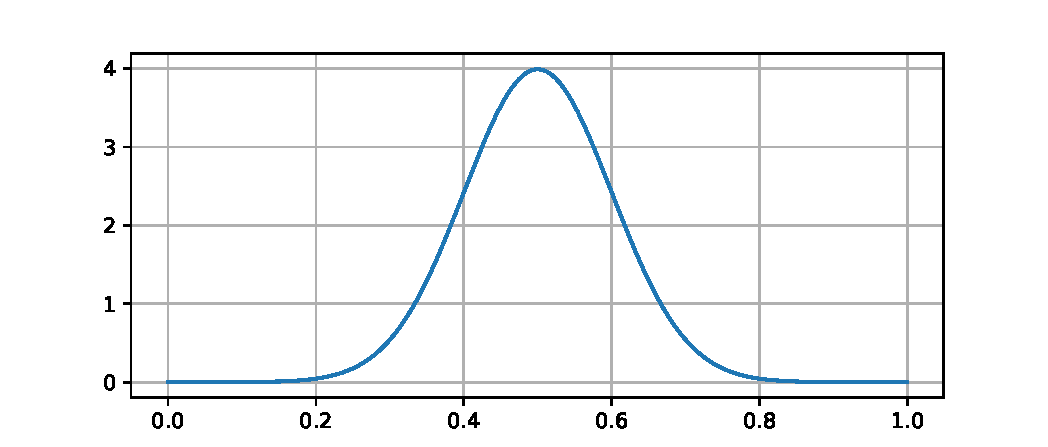
\includegraphics[width=\textwidth]{time.pdf}
    \caption{Time processing}
    \label{fig:unixtime}
\end{figure}
% data cleaning
% normalizing

% \section{Building and training}

% \subsection{Process and Select Features}
% general model, incentive: need enough data!
% Table over features

% \subsection{Generate Dataset}
% create dataset for lstm cells - lags 3 dims
% normalization of data
% create labels

% \section{Model Training and Evaluation}

% \section{Application}
% Trading strategy?
% sell if pd
% possible to buy before?
% train the model after it is deployed